% NSF proposal generation template style file.
% based on latex stylefiles written by Stefan Llewellyn Smith and
% Sarah Gille, with contributions from other collaborators.
%
\documentclass{proposalnsf}

% See this file for a set of pre-defined journal abbreviations
\newcommand{\jas}{{\it J. Atmos. Sci.}}
\newcommand{\jpo}{{\it J. Phys. Oceanogr.}}
\newcommand{\JPO}{{\it J. Phys. Oceanogr.}}
\newcommand{\jfm}{{\it J. Fluid Mech.}}
\newcommand{\jgr}{{\it J. Geophys. Res.}}
\newcommand{\JGR}{{\it J. Geophys. Res.}}
\newcommand{\jmr}{{\it J. Mar. Res.}}
\newcommand{\arfm}{{\it Ann. Rev. Fluid Mech.}}
\newcommand{\dsr}{{\it Deep-Sea Res.}}
\newcommand{\dao}{{\it Dyn. Atmos. Oceans}}
\newcommand{\jam}{{\it Journal of Applied Meteorology}}
\newcommand{\phfl}{{\it Phys. Fluids}}
\newcommand{\phfla}{{\it Phys. Fluids A}}
\newcommand{\PhilTrans}{{\it Philosophical Transactions of the Royal Society, London}}
\newcommand{\gafd}{{\it Geophys. Astrophys. Fluid Dyn.}}
\newcommand{\gfd}{{\it Geophys. Fluid Dyn.}}
\newcommand{\PCE}{{\it Physics and Chemistry of the Earth}}
\newcommand{\PRL}{{\it Physical Review Letters}}
\newcommand{\ProgOc}{{\it Prog. Oceanography}}
\newcommand{\WHOITR}{Woods Hole Oceanographic Institution Technical Report, WHOI-}


\newcommand{\degrees}{$\!\!$\char23$\!$}
\renewcommand{\refname}{\centerline{References cited}}

% This handles hanging indents for publications
\def\rrr#1\\{\par
\medskip\hbox{\vbox{\parindent=2em\hsize=6.12in
\hangindent=4em\hangafter=1#1}}}

\pagestyle{myheadings}
\usepackage{graphicx}
\graphicspath{{./figures/}}

\def\baselinestretch{1}

\begin{document}



\begin{center}

{\Large{PCA-Based Animal Classification}\\*[4mm]
{with K-Nearest Neighbors}}\\*[4mm]
{\bf CSE6363 - Final Project} \\*[4mm]

Bardia Mojra

05/15/2021

\end{center}

\noindent
{\bf Introduction}

In computer vision, we are often tasked with the classification of animals or
objects but such tasks could be cumbersome or process-heavy due to the size of
each image and the entire dataset used. In this project, I use principal component analysis (PCA) as means to extract features from the original images.
PCA has been a prominent technique for data compression and face or object
recognition, \cite{turk1991eigenfaces}. In this experiment, I use PCA to
compress the dataset and use K-Nearest Neighbors (KNN) for classification. For
the purposes of this experiment, I use the Animals-10 dataset,
\cite{Animals112:online}, and selected four classes, dog, horse, chicken, and sheep.
\ \\

\noindent
{\bf Background}

PCA became popular widely popular with the introduction of the EigenFaces
algorithm, \cite{turk1991eigenfaces}, that showed how low-resolution images
retain most relevant information that is associated with detection and
recognition of target entity, whether faces or animals, \cite{8567256}.
PCA is based on EigenValues and
EigenVectors calculated over the entire dataset. For simplicity, I explain the
following only in terms of 1D datum and 2D data set, but same applies to higher
dimensions as well. EigenVectors represent the slope
(or orientation in higher dimension) of a transform line that is normal to
variance of principal component. EigenValues represent the weight or scale of
corresponding EigenVectors which together must equal the original vector or data
set. It is also important to note each principal component tries to capture or
account for as much information as possible, therefore we expect to see
EigenValues decrease for latter EigenVectors. Figure 1 demonstrates this phenomena.

\begin{figure}[h]
  \caption{Initial Principal Components Capture The Most Information}
  \centering
  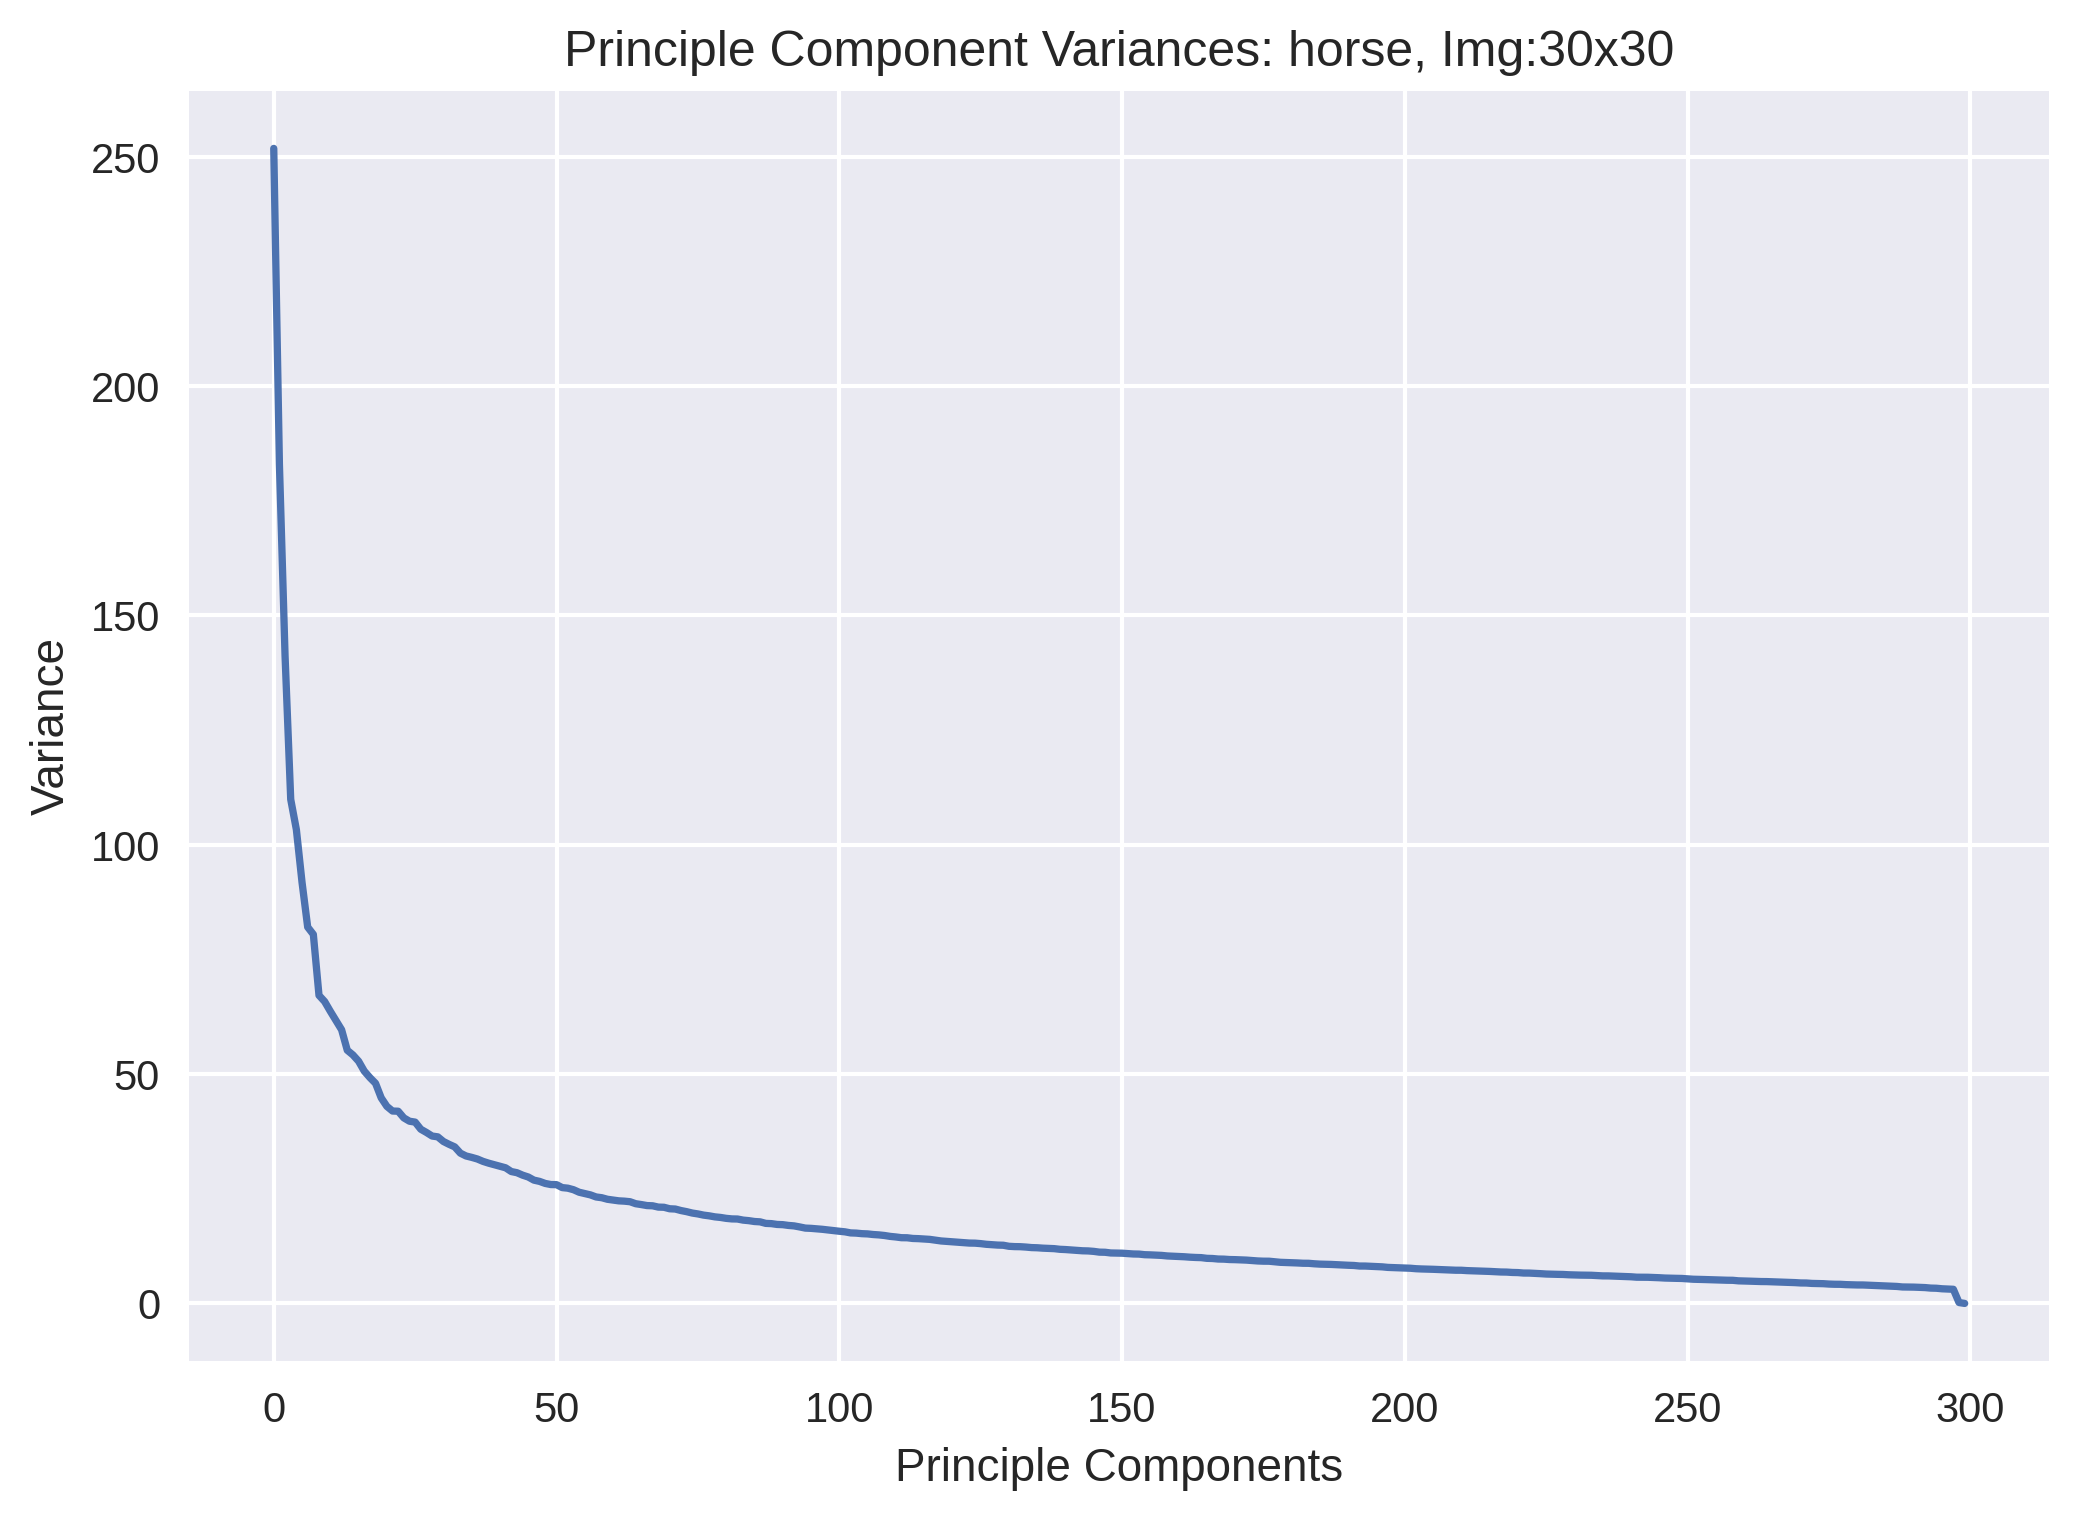
\includegraphics[width=7cm, height=6cm]{fig01}
\end{figure}


\ \\

\noindent
{\bf Method}

For implementation, first, I resized all images to nxn squares through bicubic
interpolation resampling. Images were flattened to 1x(nxn) row vectors and stacked to form our entire dataset (training + test data). To achieve faster
and proportional learning of principal components I normalized and standardized
the dataset. Using Singular Value Decomposition (SVD), I captured the dataset's
sorted EigenVectors and Covariance matrix. Since I used NumPy's built-in libraries, the returned EigenVectors were already sorted. At last, I computed
the dot product of the dataset and the EigenVectors and used it as my new dataset which is in principal component feature domain. It is import to note
we have not yet split the dataset to training and testing subsets. All mentioned steps must be performed on the entire dataset (training and test).


\begin{figure}[h]
  \caption{Initial Image Representation in Principal Component Feature Domain}
  \centering
  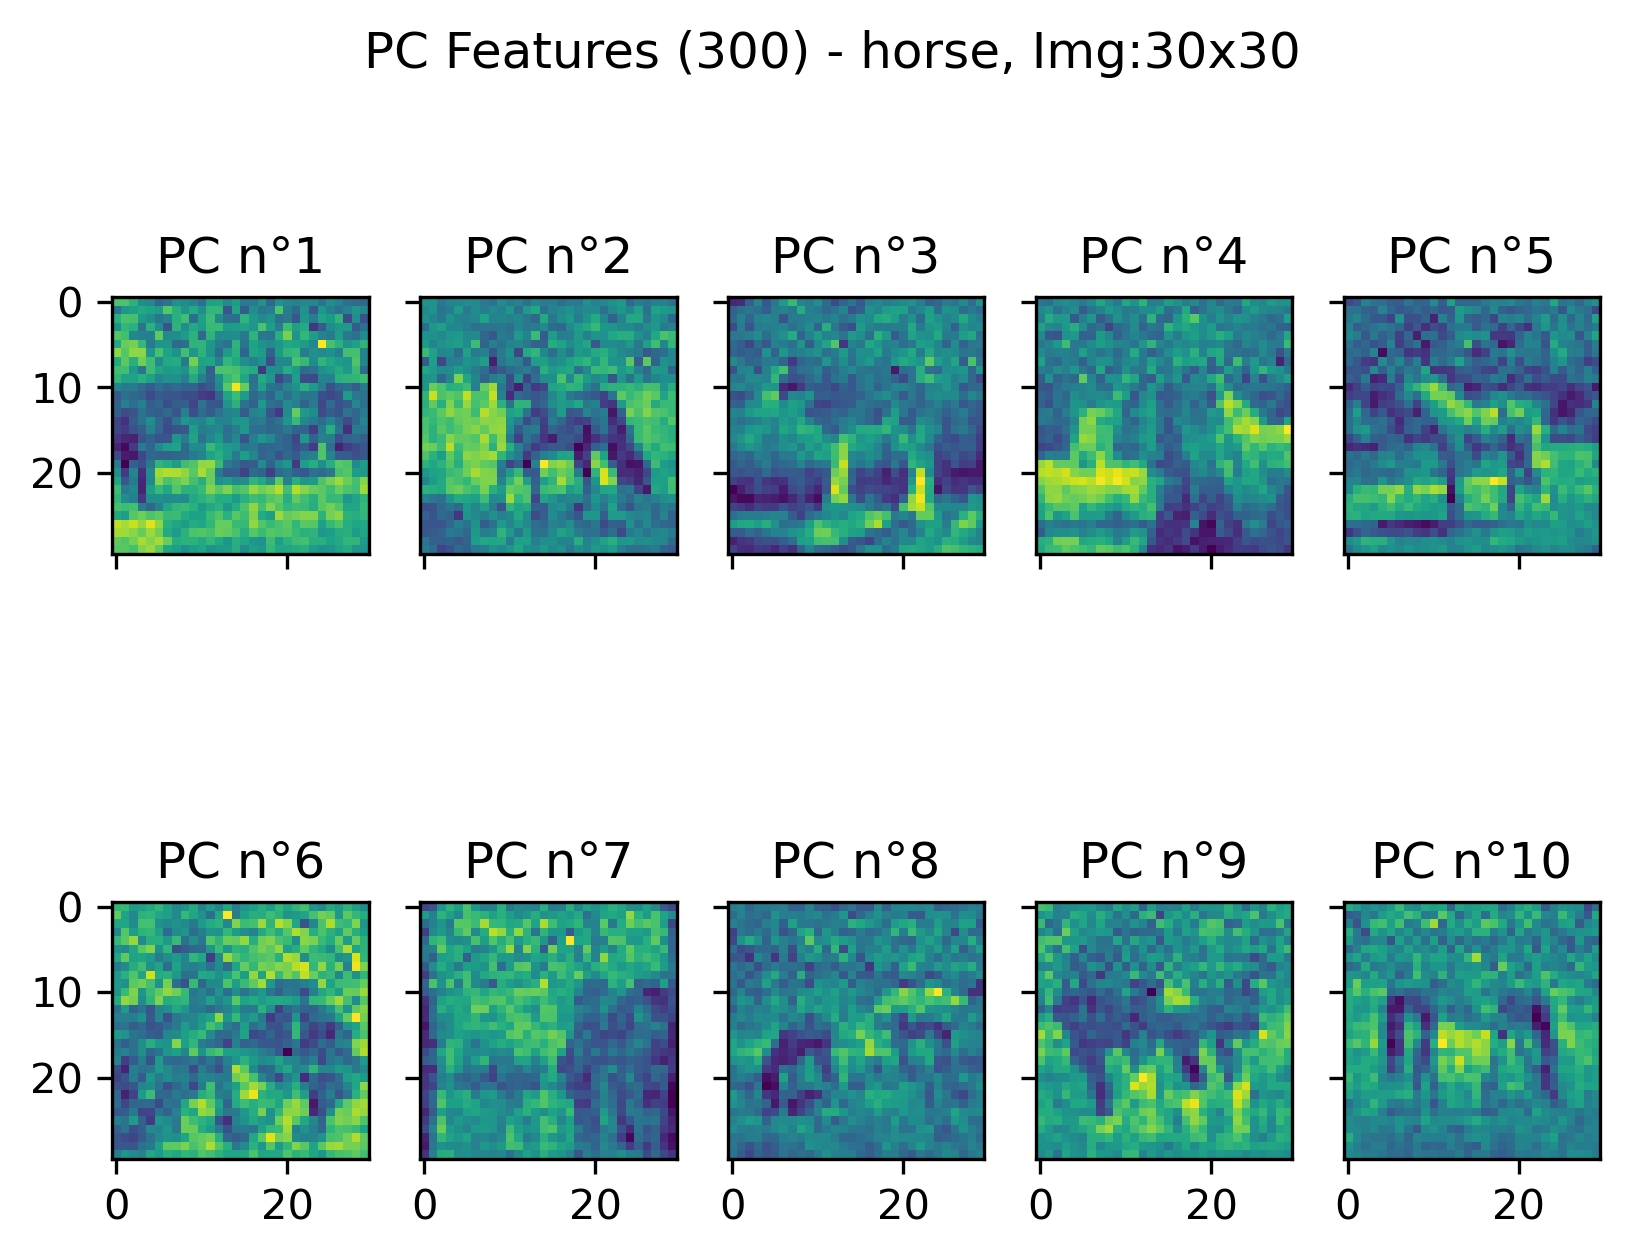
\includegraphics[width=10cm, height=7cm]{fig02}
\end{figure}


\ \\

Next, I split the dataset to 80/20 ratio for training and testing respectively.
I used KNN scheme for animal classification with k=7 and Euclidean distance was
implemented to compute the similarity score between test datum and training
data. Moreover, to improved accuracy I implemented a weighted voting scheme
at the end of KNN selection process where it takes into account the inverse
distance to k nearest neighbors.

\ \\


\noindent
{\bf Experiments}

For testing purposes, I performed over 30 experiments at various resolutions and Principal Component Ratios. The experiments were performed at 20x20, 30x30,
and 48x48 pixel resolution. Moreover, experiments were performed PCA level 5\%,
10\%, 30\%, 60\%, and 100\% of all extracted PCA's. This is to show how
representative PCA's are at each level.


There are equal number of class representation (300 per class) and classes
were shuffled ten times with uniform distribution prior to split. Since the dataset was shuffled, training and test subsets end up with different elements
when preforming each experiment; I found it important to run 10 experiments
with same configuration to capture its variance.


\ \\

\noindent
{\bf Results}

For each experiment configuration, I performed 4 tests: training data with
weighted voting, training data with simple voting, test data with weighted
voting and test data with simple voting. There is a pattern between
these four cases that that is consistent in all 30 configurations. The accuracy decrease between these four cases in order there were mentioned.

In all 30 experiment cases, test with training data with weighted voting
consistently achieve 100\% accuracy where testing on training data with simple
voting never achieve higher 97.6\% (experiment 21).

I decided to compare test cased based on percentage of PCA used rather than
the number of PC's used because the experiments where conducted at different
resolutions and higher resolution images require more principal components to
capture most relative information. By doing so, it seems that the performance
does not drop significantly if PC ratio remains constant (experiments 4, 9-18,
26). This is difficult to determine precisely unless a large number of
experiments are performed to capture the true expected value. As observed in
accuracy in experiments 4 and 26 are within the range of accuracy results from
experiments 9-18. Experiments 9 to 18 have the same configuration and were
repeated to capture the variance within the model.

The various the model is due to random nature of the reshuffling the data and
with datum is captured in the training data and in what order as initial PC's
try to account to as much information as possible, giving them higher weight
to influence prediction of the model. Model variance has a range of 7-8\%
for same repeated experiments.

Moreover, there is a clear pattern where as PC ratio is lowered, the model
accuracy decreases as well. I was able to record 76.25\%, 86.25\%, 90.83\%,
96.25\% accuracy for 20x20 pxl images with 5\%, 10\%, 30\%, and 40\% PC ratios
respectively. The pattern is clear and reasonable but to be able make more accurate conclusion more repeated tests need to be performed and average the accuracy values. Please refer to Appendix-A for a brief experiment results.


\newpage

\noindent
{\bf Appendix-A}

Please refer to document Appendix\_A.pdf.


\newpage

\bibliography{ref}
\bibliographystyle{jponew}



\end{document}
